\documentclass[10pt,conference]{IEEEtran}

% Conference class (no compsoc / compsocconf).
% Re-enable first-page \thanks (locked in conference mode by default).
\IEEEoverridecommandlockouts
\usepackage{graphicx}
\usepackage{booktabs}
\usepackage{cite}
\usepackage{url}
\usepackage{hyperref}
\usepackage{array}
\hypersetup{hidelinks}

\begin{document}

\title{Beyond Multiplier Myths: A Boundary-Aware Dual-Lens Reporting Scheme for Industrial AI4SE Pilots%
\thanks{J.~Qiu is Principal AI4SE Consultant at Inspire Group (Ph.D., Software Engineering, Tongji University; 18+ years in software engineering, R\&D productivity, and enterprise architecture).
Q.~Yan is AI4SE Engineering Advisor at Inspire Group (M.S., Computer Science, Sichuan University; 10+ years in enterprise architecture, DevOps, and AI-agent engineering).
Inspire Group is a technology-services firm formed from the former Thoughtworks China business after its acquisition by Hillhouse Capital (announced 2025); the Inspire authors facilitated the Org-A engagement.
The industrial partner remains anonymized as Org-A; no client co-authors.}}

% Inspire Group authors only; client declined co-authorship (2026-09 decision). Body keeps Org-A anonymization + sector-type portrait.
% Client legal name mapping (internal only) lives in client-disclosure-checklist.md — never in this file.
\author{
\IEEEauthorblockN{Juan Qiu\IEEEauthorrefmark{1},
Qilong Yan\IEEEauthorrefmark{1}}
\IEEEauthorblockA{\IEEEauthorrefmark{1}Inspire Group, China\\
Emails: juan.qiu@inspiregroup.com,~qlyan@inspiregroup.com}
}

\maketitle

\begin{abstract}
Enterprise sponsors of AI-for-software-engineering (AI4SE) programs often demand a single developer-productivity ``N$\times$'' multiplier, yet slogans rarely separate belief from measured delivery.
Multi-dimensional guidance such as SPACE and DORA already warns against collapsing activity, efficiency, and system delivery into one number, but transformation leaders still lack a \emph{management-usable} dual reporting protocol that jointly publishes capability change and delivery signals under disclosure limits, with explicit estimate-versus-measured labels.
We \textbf{propose} a dual-lens scheme and \textbf{illustrate} it in one industrial experience at Org-A ($\sim$6-week enablement pilot)---not a completed design-science evaluation or action-research intervention.
Lens~1 is facilitator-guided capability maturity before/after (\texttt{process\_signal}).
Lens~2 is a workshop on throughput and cycle time (CT) under a fixed Product Backlog, team, and iteration timebox (\texttt{expert\_estimate}).
A third label, \texttt{req\_measured}, is reserved for the same Throughput/CT metrics computed later from Org-A's \emph{requirements management platform} (Product/Sprint Backlog workflow; Git only where commit timestamps are needed) during real iterations; this paper does \emph{not} yet report those platform rows.
\emph{Boundary-aware} means every published cell carries a signal-type label; the estimate$\rightarrow$measured \emph{promotion path} means workshop medians stay promissory until matching \texttt{req\_measured} values validate or refute them.
At Org-A, \textbf{both} workshop Before and After were expert estimates (estimate-to-estimate): maturity lifts were modest ($+0.33$ to $+1$ on a 1--5 mean), while six pairs' median throughput improve $\Delta$ was $1.017544$ ($\approx{+}102\%$ $\sum$ story points in-window) and CT speed-improve medians were $\approx 1$---explicitly promissory expectations, not causal effect sizes or platform-validated ROI.
\end{abstract}

\begin{IEEEkeywords}
AI for software engineering, developer productivity, SPACE, DORA, maturity assessment, industrial experience report
\end{IEEEkeywords}

%% ========================================================================
\section{Introduction}
\label{sec:intro}
% Cite seeds after verification only: e.g. Forsgren2021SPACE, METR2025AIProductivity

Industry narratives about AI coding assistance often collapse value into a single multiplier---``$N\times$ faster,'' ``thousands of percent improvement,'' or similarly non-comparable slogans.
Multi-dimensional views of developer productivity caution against that collapse~\cite{Forsgren2021SPACE}: activity, communication, efficiency, and satisfaction can move in different directions, so a single throughput slogan is a management hazard rather than a decision aid.
Field and enterprise evidence on generative AI coding assistance typically reports \emph{moderate, conditional} gains---for example, roughly $26\%$ more completed tasks in pooled field experiments~\cite{Cui2026GenAIField} and about $21\%$ shorter time on a complex enterprise task in an RCT preprint~\cite{Paradis2024GoogleAISpeed}---while controlled coding tasks can show larger speedups~\cite{Peng2023Copilot}.
System-level delivery metrics popularized by DORA research (lead time, deployment frequency, change fail rate, time to restore) complement story-level throughput and cycle time; they answer different management questions~\cite{Forsgren2018Accelerate}.
Perception can diverge sharply from measured effect: experienced open-source developers in one early-2025 study expected speedup yet were slower on measured tasks~\cite{METR2025AIProductivity}.
Yet transformation sponsors still ask consultants and engineering leaders for a defensible answer to ``how much did we improve?'' under real disclosure and instrumentation constraints.

The industrial problem is therefore not the absence of any productivity literature, but the absence of a \emph{management-usable reporting scheme} that (i)~separates capability change from delivery-outcome \emph{signals}, (ii)~labels how each number was obtained, and (iii)~refuses to treat workshop consensus as platform-measured ROI.
Single-metric ``same work, faster'' framings break down when AI4SE changes how work is decomposed, verified, and shipped: the measurement space itself shifts.
Story-point volume, cycle-time endpoints, and maturity rubrics must be held fixed \emph{by protocol} if Before/After comparisons are to mean anything; otherwise teams re-point work, change iteration timeboxes, or conflate coding activity with delivery outcomes.

We address two research questions framed as empirical findings in one industrial pilot (not as method-construction prompts alone):
\begin{itemize}
\item \textbf{RQ1.} In an AI4SE enablement pilot, how do capability-maturity signals and delivery-result signals diverge in timescale and magnitude?
\item \textbf{RQ2.} When workshop Before and After conditions are both expert estimates under a fixed Product Backlog---rather than platform-measured histories---what boundaries keep dual-lens management reporting honest?
\end{itemize}

\textbf{Methodological stance.}
This manuscript is an \emph{industrial experience report}: a single-case illustration of a dual-lens reporting protocol under disclosure constraints~\cite{Runeson2009CaseStudy}.
The protocol itself is a designed artifact in the sense of design-science research~\cite{Hevner2004DSR}, but we do \emph{not} claim a complete design-science evaluation cycle, multi-case theoretical saturation under case-study guidelines~\cite{Runeson2009CaseStudy}, or an action-research intervention with researcher-owned change agency.
We report what Org-A's pilot made observable under the protocol, including modest maturity movement and promissory workshop $\Delta$s, and we foreground threats where evidence is thin.

\textbf{Contributions.} This paper contributes:
(1)~a diagnosis of why multiplier myths fail as management evidence under AI4SE (measurement-space misalignment plus missing signal-type labels);
(2)~a dual-lens \emph{reporting} scheme---capability maturity (\texttt{process\_signal}) plus Throughput/Cycle-Time signals with a three-way \texttt{signal\_type} taxonomy (two instantiated at Org-A; \texttt{req\_measured} reserved) and three design anchors (comparability, separability, honesty);
(3)~a single-case illustration at Org-A ($\sim$6-week enablement pilot) with every table number frozen in a public derived-data pack; and
(4)~managerial implications: a dual-track dashboard, an estimate$\rightarrow$measured promotion path, explicit falsifiers, and threats to validity.
We deliberately do \emph{not} claim a new RCT effect size, a scale-out ROI, a completed platform-measured closed loop at Org-A, or a universal maturity-model theory.
The transferable artifact is the reporting discipline; After-condition productivity rows in this case are workshop elicitations, not measured delivery histories.

\textbf{Incremental delta.} Relative to SPACE-style multi-dimensional caution~\cite{Forsgren2021SPACE}, DORA delivery metrics~\cite{Forsgren2018Accelerate}, and emerging AI-assisted SE maturity models~\cite{Tereci2026AASD,Garousi2025AI4SEMM,Anderson2026ACMM}, our niche is narrower: a consulting-embedded protocol that \emph{jointly} publishes maturity before/after and stratified workshop outcome signals under disclosure constraints, with an explicit estimate-vs-measured promotion path and a public derived pack for every reported cell---not a new org-wide maturity theory, nor a multi-site causal evaluation.

%% ========================================================================
\section{Industrial Context}
\label{sec:context}
% Client name in body: Org-A only.

Org-A is a large global container-shipping and logistics enterprise with a substantial, multi-site in-house IT / software-engineering organization that builds and operates enterprise-scale applications supporting core commercial, customer-facing, and operational processes.
Software delivery follows a multi-team agile model, with Product Backlog Items (PBIs) managed in a shared requirements management platform and a conventional Dev/BA/QA role split.
% Portrait uses sector-type cues only; legal client name withheld (Anon pack; client declined Named disclosure / co-authorship).
% Requirements management platform hosts Product/Sprint Backlogs and work-item workflow; not a named vendor claim.
% Workshop fixes the Product Backlog (PBI list), not the platform itself as the measurement artifact.
It ran a short, approximately six-week AI4SE enablement pilot---a phase-one explore / co-working engagement with a consulting facilitation team, not a scale-out program.
Delivery work on a pilot vehicle served as a \emph{validation context} for method enablement and evidence collection; phase success was not defined as ``scale-ready.''
Baseline tooling included conventional IDE-centric development with emerging AI assistants; the pilot introduced a spec-driven method pack (playbook, executable recipes, and facilitation rituals) rather than a single vendor coding agent alone.
Stakeholders for the executive readout included a sponsor circle (engineering leadership) and delivery leads from the pilot team; they repeatedly asked for productivity proof suitable for funding and phase-gate discussion.
\textbf{Quality as a precondition, not a missing track.}
At Org-A, product quality was already treated as a standing red line in sponsor discussions: AI4SE enablement was framed as accelerating delivery \emph{efficiency under non-degrading quality}, not as trading quality for speed.
The engagement therefore did not commission a parallel quality-instrumentation workstream for this paper; facilitators defaulted to Org-A's existing quality gates and indicators (e.g., defect escape rate and defect density under the client's established definitions) rather than inventing a new quality scoreboard beside Throughput/CT.
Those quality indicators are acknowledged as governance constraints here; this manuscript does not re-analyze or claim measured quality deltas.

The engagement's relevant outputs for this paper were: (i)~a facilitator-guided maturity re-assessment before and after the enablement window; (ii)~a facilitated effectiveness workshop under fixed Product Backlog (identical PBIs), team size, and iteration window (timebox); and (iii)~an executive readout that stated signal-type boundaries to management.
Those questions are legitimate; answering them with a single invented multiplier is not.
The consulting response was a dual-lens reporting scheme rather than a slogan contest.
Workshop expert estimates were positioned as promissory expectations under high method consensus, not as platform-measured ROI; modest maturity movement over a few weeks was treated as an expected finding rather than a narrative failure.
Explicit non-claims were recorded for the phase: phase success $\neq$ scale-ready; expert-estimate workshop results $\neq$ platform-measured ROI.

\textbf{Why a dual lens was required.}
A maturity-only story would under-answer the ``how much throughput / cycle time?'' ask; a workshop-only story would ignore whether capabilities were being institutionalized.
Reporting both with different \texttt{signal\_type} labels lets sponsors track process and result expectations without forcing them onto one scale.

For anonymity, the client is labeled Org-A only; workshop groups appear as Pair-1\ldots Pair-6; no participant or facilitator personal names appear in this paper or in the accompanying public-data pack.
Identifiable product features from the pilot vehicle are also withheld.
Workshop participation was part of an industrial enablement engagement; published materials use only anonymized pair IDs and derived aggregates. Conference submission will include the venue's human-participants compliance declaration.

%% ========================================================================
\section{Measurement Scheme}
\label{sec:scheme}
% PLANNED FIGS: S1 dual-lens + signal_type layers; S2 workshop protocol

The scheme answers two management questions on one dashboard: \emph{Are capabilities moving?} and \emph{What throughput / cycle-time improvement can we expect under high consensus?}
Every published row carries a \texttt{signal\_type} (Table~\ref{tab:signal-types}).
Every protocol choice traces to one of three anchors (Table~\ref{tab:anchors}).

\begin{table}[!t]
\centering
\caption{Signal-type taxonomy used in reporting.}
\label{tab:signal-types}
\footnotesize
\setlength{\tabcolsep}{3pt}
\begin{tabular}{@{}>{\ttfamily\raggedright\arraybackslash}p{0.34\columnwidth}>{\raggedright\arraybackslash}p{0.60\columnwidth}@{}}
\toprule
\normalfont\texttt{signal\_type} & Meaning in this paper \\
\midrule
expert\_estimate & Facilitated SME / pair judgment---\textbf{both} workshop Before and After rows at Org-A \\
process\_signal & Expert-facilitated maturity assessment (domain/capability levels) \\
req\_measured & Same Throughput/CT metrics computed from the requirements management platform (Product/Sprint Backlog workflow; Git if needed for CT1)---\textbf{not yet reported} for Org-A Before/After in this paper \\
\bottomrule
\end{tabular}
\end{table}

\noindent{\footnotesize In this paper, \emph{requirements management platform} means Org-A's shared system for Product Backlog / Sprint Backlog items and their workflow states (optionally linked to Git for commit timestamps)---not a full Application Lifecycle Management suite claim, and not a named vendor product. The workshop's fixed work list is the Product Backlog (identical PBIs for all pairs), hosted on that platform.}

\begin{table}[!t]
\centering
\caption{Signal-type legend (used throughout tables and figures).}
\label{tab:signal-legend}
\scriptsize
\setlength{\tabcolsep}{2pt}
\begin{tabular}{@{}>{\ttfamily\raggedright\arraybackslash}p{0.36\columnwidth}>{\raggedright\arraybackslash}p{0.58\columnwidth}@{}}
\toprule
\normalfont\texttt{signal\_type} & Reader cue \\
\midrule
expert\_estimate & Workshop / SME judgment (promissory; Org-A Before \emph{and} After) \\
process\_signal & Facilitated maturity levels (capability change, not delivery ROI) \\
req\_measured & Same metrics from the requirements platform in real iterations (\textbf{not reported} for Org-A here) \\
\bottomrule
\end{tabular}
\end{table}

\textbf{Critical boundary: Before is also an estimate.}
Org-A is a mature agile organization with platform history, yet the workshop did \emph{not} bind Before to a historical platform window.
Both Before (traditional delivery) and After (spec-driven method at high consensus) were elicited as \texttt{expert\_estimate} on the \emph{same} fixed Product Backlog, team, and iteration timebox, so that the only intended contrast is method under those controls.
Historical platform throughput on past sprints typically does not map onto that exact PBI set and timebox; After under the new method also had no closed platform history yet.
Consequently, Before$\rightarrow$After $\Delta$ is an \emph{estimate-to-estimate} contrast (a promissory method lift)---not measured-baseline$\rightarrow$estimate, and not platform$\rightarrow$platform.
We treat that as a first-order credibility issue (Section~\ref{sec:threats}): the gap can reflect shared optimism (``imagination gap'') as well as genuine method expectation, which is why \texttt{req\_measured} validation remains mandatory before ROI language.


\begin{table}[!t]
\centering
\caption{Three design anchors for the productivity workshop.}
\label{tab:anchors}
\begin{tabular}{@{}lp{0.68\columnwidth}@{}}
\toprule
Anchor & Operational implication \\
\midrule
Comparability & Hold Product Backlog (PBI list), team size, and iteration window (timebox) constant so Before$\rightarrow$After differences are not explained by those three condition drifts (this does \emph{not} prove causal attribution to the method alone) \\
Separability & Freeze story points after joint estimation; After must not re-point \\
Honesty & Report high-consensus expert judgment as promissory expectation, not platform-measured ROI \\
\bottomrule
\end{tabular}
\end{table}

\subsection{Capability Maturity Lens}
\label{sec:scheme-maturity}
% EVIDENCE: measurement-scheme-summary.md (6 domains / 18 capabilities, L1--L5)
% signal_type for maturity scores: process_signal (not platform-measured)
% PUBLIC: public-data/protocol/maturity-scoring-guide.md

Capability maturity is assessed with a facilitator-guided instrument covering \textbf{6 domains $\times$ 18 capabilities} (3 per domain) on levels \textbf{L1--L5} (Initial $\rightarrow$ Toolized $\rightarrow$ Engineered $\rightarrow$ Systematized $\rightarrow$ Autonomous).
English domain labels used in derived data are: Efficiency Foundation; Process Layer; Engineering Methods \& Discipline; Tooling Layer; Human--Agent Collaboration; and Organization \& Culture.
Example capabilities include value goals and outcome hypotheses (D1.1), AI4SE workflow design (D2.1), spec-driven expression (D3.1), agent runtime and permissions (D4.1), human-in-/on-/out-of-the-loop risk routing (D5.2), and practice champions and training (D6.1); the full 18-item list ships in \texttt{maturity\_capabilities.csv}.

\textbf{Scoring packaging.}
A consulting facilitator walks sponsors and delivery leads through each capability against short L1--L5 anchors (observable practice cues), records a consensus level, and revisits the same instrument after the enablement window.
At Org-A, Before and After scores were collected by the same facilitation team around the start and end of the $\sim$6-week pilot; the effectiveness workshop was a separate session under fixed conditions and is \emph{not} the maturity instrument.
The public pack includes a concise scoring guide (\texttt{maturity-scoring-guide.md}) with level anchors and facilitation notes; it is an industrial rubric for repeated use, not a psychometrically validated scale.
No inter-rater reliability study is claimed here: scores are expert-facilitated consensus under time pressure.

\textbf{Ordinal caveat.}
Domain means in tables are convenience averages of three ordinal levels on a 1--5 encoding; they support before/after narrative comparison within this instrument, not interval-scale inference or cross-vendor maturity rankings.
A $+0.33$ domain mean typically reflects a one-level lift on a single capability with the other two unchanged.

Scores are labeled \texttt{process\_signal}: they track organizational capability change, not product quality or business outcome, and they are \emph{not} platform-measured.
The instrument is intended for repeated assessment across transformation phases; a short pilot should be expected to move only a subset of capabilities by one level.
Relative to emerging AI-assisted SE maturity models that emphasize governance, competency, and feedback infrastructure~\cite{Tereci2026AASD,Garousi2025AI4SEMM,Anderson2026ACMM}, this lens is a \emph{program-local} 6$\times$18 checklist for dual-track reporting---not a replacement org-wide maturity theory.

\subsection{Productivity Signal Lens}
\label{sec:scheme-productivity}
% EVIDENCE: measurement-scheme-summary.md; metrics-definitions.md; workshop-protocol.md
% Anchors: comparability / separability / honesty
% signal_type $\in$ \{expert\_estimate, process\_signal, req\_measured\}

\textbf{Throughput.}
In the metrics specification, $\mathrm{Throughput}=\sum(\mathrm{SP\ of\ completed\ stories\ in\ window})/\mathrm{PersonDays}$ (points / person-day).
Here \emph{window} denotes the fixed agile \emph{iteration timebox} used by the workshop (not the multi-week enablement pilot).
Completion is the first transition to QA testing completed (or platform-equivalent).
Under the workshop's fixed team $\times$ iteration window, PersonDays is approximately constant, so \textbf{$\sum$ SP} in the window is the primary floor report and is monotone-equivalent for Before/After $\Delta$.

\textbf{Cycle time (CT).}
We write \textbf{CT} for \emph{cycle time}: the elapsed duration of a story between two defined platform workflow endpoints (not the iteration timebox, and not DORA lead time for changes).
The workshop primary-reports two story-level CT variants (Table~\ref{tab:ct-variants}):
\begin{itemize}
\item \textbf{CT1} (\emph{code} cycle time; spec alias $\mathrm{CT_{code}}$): from DEV accept to the latest related commit---coding-centric elapsed time.
\item \textbf{CT2} (\emph{delivery} cycle time; spec alias $\mathrm{CT_{delivery}}$): from the same DEV-accept start to QA testing completed---includes handoff into test-done.
\end{itemize}
$\mathrm{CT_{prod}}$ (to production release) is defined in the metrics spec but not primary-reported on the floor (non-dev release noise).
Within-pair CT summaries use \textbf{P75} at story grain.
After (spec-driven) work may be planned as Changes, but statistics fold back to stories before P75.

\begin{table}[!t]
\centering
\caption{Cycle Time (CT) variants used in the workshop.}
\label{tab:ct-variants}
\footnotesize
\setlength{\tabcolsep}{2pt}
\resizebox{\columnwidth}{!}{%
\begin{tabular}{@{}>{\raggedright\arraybackslash}p{0.11\columnwidth}>{\raggedright\arraybackslash}p{0.26\columnwidth}>{\raggedright\arraybackslash}p{0.59\columnwidth}@{}}
\toprule
CT & Meaning & Endpoints (start $\rightarrow$ end) \\
\midrule
CT1 & Code ($\mathrm{CT_{code}}$) & DEV accept $\rightarrow$ latest related commit \\
CT2 & Delivery ($\mathrm{CT_{delivery}}$) & DEV accept $\rightarrow$ QA testing completed \\
\bottomrule
\end{tabular}}\\[0.3em]
{\scriptsize DEV accept $=$ first Product Backlog $\rightarrow$ Required Analysis transition on the story. CT$*$ durations are story-grain; pair summaries use P75.}
\end{table}

\textbf{Paired improve $\Delta$.}
Throughput improve is $(\mathrm{TP_{after}}-\mathrm{TP_{before}})/\mathrm{TP_{before}}$.
CT speed improve (primary narrative) is $(\mathrm{CT_{before}}-\mathrm{CT_{after}})/\mathrm{CT_{after}}=\mathrm{speedup}-1$ for the chosen CT variant (CT1 or CT2); we also report speedup $\mathrm{CT_{before}}/\mathrm{CT_{after}}$ and duration reduction $(\mathrm{CT_{before}}-\mathrm{CT_{after}})/\mathrm{CT_{before}}$, without conflating denominators.
Cross-pair primary claims use the \textbf{median and IQR} of the six pair $\Delta$s---not the mean of means, and not the maximum pair.

\textbf{Workshop protocol (fixed conditions).}
Table~\ref{tab:workshop-fixed} summarizes the fixed conditions.
Twelve participants form \textbf{six independent pairs} (Pair-1\ldots Pair-6) that estimate Before (traditional delivery) vs.\ After (spec-driven method pack at high consensus) without mid-workshop sharing, to limit anchoring.
Stages: (1)~clarify Product Backlog PBIs \& freeze SP (read-only thereafter); (2)~Before estimates of which stories finish in the iteration window and story-level CT1/CT2; (3)~After estimates (scope as Changes, map back to stories, sum \emph{frozen} SP, recompute P75 CT); facilitator aggregates six pair $\Delta$s into median / IQR (and optionally min/max).
The protocol forbids averaging all Before then all After into one global $\Delta$, and forbids dropping pairs for ``ugly'' numbers except for documented protocol violations.
All effectiveness rows are \texttt{expert\_estimate}.

\begin{table}[!t]
\centering
\caption{Fixed workshop conditions (comparability).}
\label{tab:workshop-fixed}
\footnotesize
\setlength{\tabcolsep}{2pt}
\begin{tabular}{@{}>{\raggedright\arraybackslash}p{0.34\columnwidth}>{\raggedright\arraybackslash}p{0.60\columnwidth}@{}}
\toprule
Condition & Workshop setting \\
\midrule
Product Backlog & Identical PBI list for all pairs (platform-hosted backlog; SP frozen after Stage~1) \\
Team size & Fixed roster (study example: 5 Dev + shared BA/QA fractions) \\
Iteration window & Agile iteration timebox: 2 weeks / 10 working days \\
Story points & Frozen after Stage-1 joint estimation; After must not re-point \\
\bottomrule
\end{tabular}
\end{table}

\subsection{Combined Management Dashboard}
\label{sec:scheme-dashboard}
% EVIDENCE: measurement-scheme-summary.md (dual-track narrative)
% Reading rule: modest maturity $\neq$ failure; workshop estimate $\neq$ platform-measured ROI.

Table~\ref{tab:dashboard} states the joint reading rule.
Track both lenses with explicit \texttt{signal\_type} labels; never substitute estimate for measured ROI; never treat flat maturity as ``no value'' when method assets and promissory expectations still exist.
Operationally, the dashboard is a \emph{two-track} artifact: one track is capability levels over time; the other is stratified productivity signals with the estimate$\rightarrow$measured promotion path reserved for \texttt{req\_measured} rows that do not yet exist for Org-A's After condition.
The closed loop for later phases is: publish workshop medians as expectations, then validate or refute them with \texttt{req\_measured} telemetry under the same metric definitions.
A third anti-pattern to avoid is mixing denominators---reporting duration reduction $\%$ as if it were speed-improve $\%$---which the protocol tables explicitly separate.

\begin{table}[!t]
\centering
\caption{Dual-lens management dashboard (reading rules).}
\label{tab:dashboard}
\footnotesize
\setlength{\tabcolsep}{2pt}
\begin{tabular}{@{}>{\raggedright\arraybackslash}p{0.34\columnwidth}>{\raggedright\arraybackslash}p{0.60\columnwidth}@{}}
\toprule
Lens & Honest read \\
\midrule
Maturity & Modest short-pilot movement is an expected finding, not automatic failure \\
Productivity signals & Workshop $=$ promissory expectation under fixed conditions; close the loop later with \texttt{req\_measured} \\
Joint use & Capability lift $\neq$ ROI; estimate $\neq$ platform-measured; keep both tracks labeled \\
\bottomrule
\end{tabular}
\end{table}

\textbf{Coverage vs.\ SPACE and DORA (deliberate omissions).}
SPACE warns that Satisfaction, Performance, Activity, Communication/collaboration, and Efficiency/flow can diverge~\cite{Forsgren2021SPACE}; this scheme operationalizes primarily Efficiency/flow (Throughput, CT) plus a process-capability track, and does \emph{not} claim DevEx satisfaction surveys, communication-network metrics, or a new quality/defect Performance instrument as primary Org-A rows.
That omission is not a claim that quality is unimportant: Org-A sponsors treated quality as a default, non-negotiable constraint (Section~\ref{sec:context}), and AI4SE efficiency asks were posed under ``quality must not degrade.''
Accordingly, the pilot retained the client's existing quality requirements (illustratively defect escape rate and defect density) instead of adding a separate workshop quality lens; this paper simply does not expand those retained indicators.
DORA-style system metrics (deployment frequency, lead time for changes, change fail rate, time to restore)~\cite{Forsgren2018Accelerate} likewise remain out of the workshop primary report: CT1/CT2 are story-grain delivery intervals under a fixed Product Backlog and iteration timebox, not org-level change lead time or reliability.
Sponsors who need SPACE satisfaction, DORA reliability, or a published quality before/after pack must instrument those tracks separately; omitting them here is intentional under disclosure, cadence, and the client's ``quality already governed'' stance---not a claim that Throughput/CT alone suffice for all management decisions.

\textbf{Sponsor decision tree (anti-misquote).}
When maturity $\Delta$ is modest and workshop medians are large---the Org-A pattern---sponsors should: (1)~fund next-phase method enablement and instrumentation, not declare ROI; (2)~schedule \texttt{req\_measured} validation against the same definitions before any funding slide quotes $+102\%$ $\sum$ SP or $\approx 2\times$ CT speedup as achieved productivity; (3)~forbid retelling Pair-3 maxima as the organizational headline when the primary claim is median+IQR; (4)~ask who owns the dual dashboard (engineering leadership + delivery leads jointly) and what incentive pressure would punish honest estimate$\neq$measured divergence.
Executive-facing narrative may round to ``about $+100\%$ $\sum$ SP under workshop conditions (promissory)'' while precision stays in CSV/tables.

\textbf{Falsifiers.}
The \emph{scheme} fails if published rows drop \texttt{signal\_type}, if After re-points work, if workshop maxima replace median+IQR as primary claims, or if estimate rows are promoted to ROI without platform-measured confrontation.
The \emph{enablement} fails if later \texttt{req\_measured} $\Delta$s remain near zero under the same definitions while method consensus was claimed high, if maturity domains tied to the method pack stay flat across multiple reassessment cycles with no asset adoption evidence, or if efficiency narratives are advanced while Org-A's quality red-line indicators (e.g., defect escape / density under client definitions) are knowingly breached or dropped from governance.
Either failure is reportable news---not a reason to invent a multiplier.

\textbf{Ethics and politics of the dashboard.}
Throughput/CT estimates can become weapons in headcount or vendor debates; facilitators must keep ownership of labels with named sponsors, surface risk/DevEx beside volume when available, and treat refusal to schedule platform-measured validation as a governance red flag rather than a data gap to paper over.

\textbf{Application note (executive use).}
On one slide, report maturity domain means and workshop median+IQR, each with \texttt{signal\_type}; use maturity for ``are we building lasting capability?'' and workshop signals for ``what delivery lift should we expect under high consensus?''
Do not collapse the two into one multiplier; do not headline Pair-3 maxima when the primary claim is median+IQR; apply the decision tree above when maturity is modest and estimates are large.
Research implications of this dual-track reading appear in Section~\ref{sec:discussion}.

%% ========================================================================
\section{Case Application}
\label{sec:case}
% EVIDENCE: maturity-before-after.md; effectiveness-signals.md; E6 process slice (anon)
% NUMBERS MUST MATCH: public-data/derived/*.csv

We apply the scheme to Org-A's $\sim$6-week pilot.
All quantitative cells below are copied from \texttt{public-data/derived/*.csv}.

\subsection{Process Narrative}
\label{sec:case-process}
% EVIDENCE: org-context-anon.md; executive readout slice (E6) anonymized

Phase one followed a short enablement cadence rather than a delivery-acceptance program.
Sponsors opened with a productivity-proof ask under disclosure limits; facilitators answered with the dual-lens scheme instead of a single multiplier because Org-A already had quality red lines and an immature instrumentation path for After under the new method.

\textbf{Why these protocol choices.}
We fixed Product Backlog, team, and iteration timebox so Before/After workshop contrasts would not be explained by scope or calendar drift; we froze story points after joint estimation so After could not ``win'' by re-pointing; and we deliberately elicited \emph{both} poles as \texttt{expert\_estimate} on that same PBI list because a historical platform window would not map onto the fixed backlog used for After SDD scoping.
Those choices trade measured-baseline credibility for within-workshop comparability---a trade we surface rather than hide (Section~\ref{sec:scheme}).

\textbf{What the weeks looked like.}
A kickoff week locked diagnosis, sponsor questions, and a pilot vehicle as the validation context for method assets.
Four workshop weeks then co-created a spec-driven method pack (playbook, opportunity specs, executable recipes/skills) with the pilot team on real PBIs.
Mid-engagement, facilitators tightened wording for executive materials: phase success meant reusable method assets and bounded evidence---not ``all business scope done,'' not scale-ready, and not estimate-as-ROI.
Near the start and end of the enablement window, the same facilitation team ran the 6$\times$18 maturity re-assessment (\texttt{process\_signal}); learning-to-the-test was possible and was \emph{not} blinded in this pilot.
Separately, the effectiveness workshop (six pairs, independent estimates) produced Table~\ref{tab:effectiveness-agg}'s promissory $\Delta$s.
A closing executive readout presented both lenses with signal-type labels, retained quality gates, and a next-step path of sedimentation before any scale-out discussion.

\textbf{What we hit and did not do.}
The main friction was executive appetite for a single $N\times$ number while instrumentation for \texttt{req\_measured} After was not yet closed; the honest move was to publish estimate-to-estimate contrasts with hard labels rather than invent platform ROI.
We did \emph{not} bind workshop Before to a matched historical platform window on the same PBI set; close After with \texttt{req\_measured} telemetry; or publish a parallel quality before/after pack beyond existing client gates.

\subsection{Maturity Before/After}
\label{sec:case-maturity}
% CSV: public-data/derived/maturity_domain_scores.csv
% CSV: public-data/derived/maturity_capabilities.csv
% PLANNED FIGS: F1 (domains), F2 (capabilities) per figure_sources.json
% Honesty: short pilot $\rightarrow$ limited maturity movement is an expected finding.

Table~\ref{tab:maturity-domains} and Fig.~\ref{fig:maturity-domains} report domain means (\texttt{process\_signal}).
\textbf{Overall deltas are modest:} domain lifts range from $+0.33$ to $+1.00$; most domains remain in the low-L2 / low-L3 mean band after re-assessment.
Largest lifts: Organization \& Culture (D6, $\Delta=1$); Process Layer and Engineering Methods \& Discipline (D2, D3, $\Delta=0.66$ each).
Smaller lifts: Efficiency Foundation, Tooling Layer, and Human--Agent Collaboration ($+0.33$ each).

Capability detail (18 items in \texttt{maturity\_capabilities.csv}) shows several capabilities remaining at L2 with $\Delta=0$ (e.g., D1.1, D1.2, D2.3, D3.3, D4.2, D4.3, D5.1, D5.3).
Table~\ref{tab:maturity-cap-excerpt} excerpts capabilities with non-zero $\Delta$ to illustrate where movement concentrated.
After the pilot, D1 and D5 still have zero capabilities at L3+.
L1 shortfalls cleared in D1, D2, D3, and D5 (L1 counts $1\rightarrow0$); D6 after has three capabilities at L3+.
Tooling and verification depth did not jump to systematized levels in this window.

\begin{table}[!t]
\centering
\caption{Capability-level lifts with $\Delta\neq0$ (excerpt). All rows: \texttt{process\_signal}. Source: \texttt{maturity\_capabilities.csv}.}
\label{tab:maturity-cap-excerpt}
\begin{tabular}{@{}lllr@{}}
\toprule
ID & Capability (short) & Before$\rightarrow$After & $\Delta$ \\
\midrule
D1.3 & Efficiency \& Flow Measurement & L1$\rightarrow$L2 & 1 \\
D2.1 & AI4SE Workflow Design & L2$\rightarrow$L3 & 1 \\
D2.2 & Small-Batch Task Decomposition & L1$\rightarrow$L2 & 1 \\
D3.1 & Spec-Driven Expression & L2$\rightarrow$L3 & 1 \\
D3.2 & Context Organization & L1$\rightarrow$L2 & 1 \\
D4.1 & Agent Runtime \& Permissions & L2$\rightarrow$L3 & 1 \\
D5.2 & HITL/HOTL/HOOL Risk Routing & L1$\rightarrow$L2 & 1 \\
D6.1--3 & Champions / Community / Adoption & L2$\rightarrow$L3 & 1 each \\
\bottomrule
\end{tabular}
\end{table}

\textbf{Explicit finding:} a short ($\sim$6-week) enablement pilot $\Rightarrow$ limited maturity movement is an \emph{expected} finding, not a failure to report.
Capability curves are slow relative to workshop promissory expectations; both lenses must stay on the dual dashboard without forcing a success narrative.

\begin{table}[!t]
\centering
\caption{Maturity domain means before/after (Org-A). All rows: \texttt{process\_signal}. Source: \texttt{maturity\_domain\_scores.csv}.}
\label{tab:maturity-domains}
\begin{tabular}{@{}llrrr@{}}
\toprule
ID & Domain & Before & After & $\Delta$ \\
\midrule
D1 & Efficiency Foundation & 1.67 & 2 & 0.33 \\
D2 & Process Layer & 1.67 & 2.33 & 0.66 \\
D3 & Eng.\ Methods \& Discipline & 1.67 & 2.33 & 0.66 \\
D4 & Tooling Layer & 2 & 2.33 & 0.33 \\
D5 & Human--Agent Collaboration & 1.67 & 2 & 0.33 \\
D6 & Organization \& Culture & 2 & 3 & 1 \\
\bottomrule
\end{tabular}
\end{table}

\begin{figure}[!t]
\centering
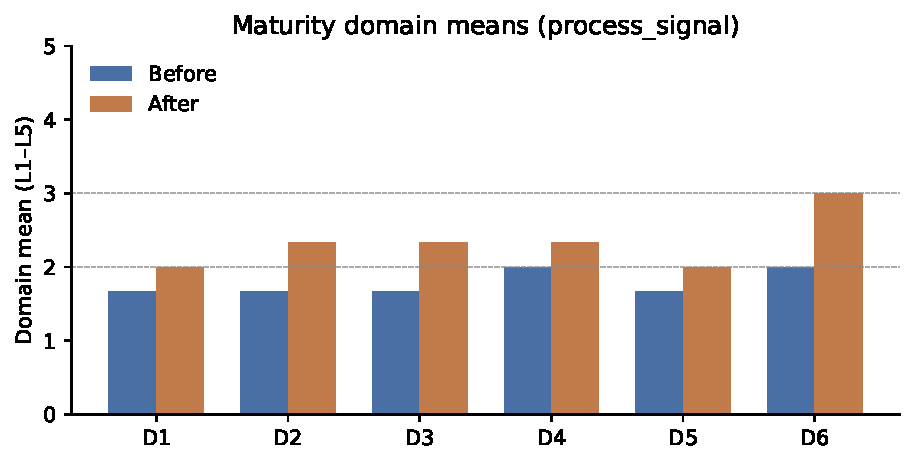
\includegraphics[width=\columnwidth]{figures/f1-maturity-domains.pdf}
\caption{Maturity domain means before/after (\texttt{process\_signal}). Horizontal guides at L2 and L3.}
\label{fig:maturity-domains}
\end{figure}

\subsection{Workshop Effectiveness Signals}
\label{sec:case-effectiveness}
% CSV: public-data/derived/effectiveness_pair_summary.csv
% CSV: public-data/derived/effectiveness_aggregate.csv
% PLANNED FIGS: F3 (pairs), F4 (median/IQR)
% All workshop rows: signal_type=expert_estimate; pairs Pair-1..Pair-6 only.

Under fixed Product Backlog / team / iteration window and frozen SP, six pairs produced Before/After estimates.
\textbf{Interpretation label (required):} promissory expectation under high method consensus---\textbf{not} measured ROI, and \textbf{not} \texttt{req\_measured}.
\textbf{Both poles are estimates:} Before (traditional delivery on the fixed PBI list) and After (spec-driven method at high consensus) are \texttt{expert\_estimate}; Table~\ref{tab:effectiveness-agg} is therefore an estimate-to-estimate contrast (Section~\ref{sec:scheme}), not an platform baseline versus a workshop forecast.

\textbf{Throughput (volume construct).}
Table~\ref{tab:effectiveness-agg} reports cross-pair aggregates for throughput improve $\Delta$ ($\sum$ SP in the iteration window): median $1.017544$ (IQR $0.039384$), range $[0.76,\ 1.472727]$.
The median fractional improve of $\approx 1.02$ corresponds to roughly $+102\%$ completed story-point volume in the fixed timebox as \emph{estimated} by pairs---about a doubling of in-window $\sum$ SP under workshop conditions, not organization-wide ROI.

\textbf{Cycle time (speed construct).}
Separately, CT1 speed-improve $\Delta$ at P75 has median $1$ (IQR $0.1875$); CT2 speed-improve $\Delta$ at P75 has median $1.018519$ (IQR $0.616402$).
Speed-improve $\Delta=(\mathrm{CT}_{b}-\mathrm{CT}_{a})/\mathrm{CT}_{a}$ equals speedup$-1$; a CT1 median of $1$ therefore corresponds to roughly $2\times$ faster P75 code cycle time under the same promissory label.
We do \emph{not} claim that throughput ``also'' sped up $2\times$: $\sum$ SP improve $\Delta$ and CT speed-improve $\Delta$ are different constructs (volume change vs.\ duration speedup) and must not be narrated as one interchangeable multiplier.
We do not cherry-pick the maximum pair for the primary claim.

Table~\ref{tab:effectiveness-pairs} summarizes pair-level throughput and CT P75.
Pair $\Delta$s vary (e.g., Pair-5 throughput improve $0.76$; Pair-3 $1.472727$), reinforcing median+IQR over max-pair storytelling.
Executive narrative may say ``about $+100\%$ $\sum$ SP (volume) and about $2\times$ CT speedup (duration), both workshop estimates''; tables keep full precision and keep the two constructs separate.

\begin{table*}[!t]
\centering
\caption{Cross-pair aggregates of improve $\Delta$ (Org-A workshop). All rows: \texttt{expert\_estimate}. CT $=$ cycle time. Source: \texttt{effectiveness\_aggregate.csv}.}
\label{tab:effectiveness-agg}
\begin{tabular}{@{}lrrrrr@{}}
\toprule
Metric & Median & IQR & p25 & p75 & Min--Max \\
\midrule
TP improve $\Delta$ & 1.017544 & 0.039384 & 1 & 1.039384 & 0.76--1.472727 \\
CT1 speed $\Delta$ @P75 & 1 & 0.1875 & 1 & 1.1875 & 0.772727--1.714286 \\
CT2 speed $\Delta$ @P75 & 1.018519 & 0.616402 & 0.75 & 1.366402 & 0.666667--1.619048 \\
\bottomrule
\end{tabular}
\end{table*}

\begin{table*}[!t]
\centering
\caption{Pair summary (workshop): throughput and Cycle Time (CT) P75. All rows: \texttt{expert\_estimate}. Source: \texttt{effectiveness\_pair\_summary.csv}.}
\label{tab:effectiveness-pairs}
\setlength{\tabcolsep}{4pt}
\begin{tabular}{@{}lrrrrrrrrr@{}}
\toprule
Pair & TP$_b$ & TP$_a$ & TP $\Delta$ & CT1$_b$ & CT1$_a$ & CT1$_{\uparrow}$ & CT2$_b$ & CT2$_a$ & CT2$_{\uparrow}$ \\
\midrule
Pair-1 & 49 & 100 & 1.040816 & 3.75 & 1.875 & 2 & 5.5 & 2.1 & 2.619048 \\
Pair-2 & 57 & 116 & 1.035088 & 3 & 1.5 & 2 & 5 & 3 & 1.666667 \\
Pair-3 & 55 & 136 & 1.472727 & 4.75 & 1.75 & 2.714286 & 6.5 & 2.625 & 2.47619 \\
Pair-4 & 45 & 90 & 1 & 4.875 & 2.75 & 1.772727 & 6.875 & 3.375 & 2.037037 \\
Pair-5 & 50 & 88 & 0.76 & 4.5 & 2 & 2.25 & 5 & 2.5 & 2 \\
Pair-6 & 50 & 100 & 1 & 4 & 2 & 2 & 5 & 3 & 1.666667 \\
\bottomrule
\end{tabular}\\[0.4em]
{\footnotesize TP$_b$/TP$_a$: $\sum$ SP before/after. TP $\Delta$: improve fraction $(\mathrm{TP}_a-\mathrm{TP}_b)/\mathrm{TP}_b$. CT$*_b$/$a$: Cycle Time P75 durations (CT1$=$code; CT2$=$delivery). CT$*_{\uparrow}$: speedup $=\mathrm{CT}_b/\mathrm{CT}_a$. Aggregate Table~\ref{tab:effectiveness-agg} uses speed-improve $\Delta=$ speedup$-1$; e.g., Pair-1 CT1$_{\uparrow}=2$ $\Rightarrow$ speed $\Delta=1$.}
\end{table*}

\subsection{Reading Both Lenses Together}
\label{sec:case-joint}
% EVIDENCE: maturity-before-after.md; effectiveness-signals.md; measurement-scheme-summary.md
% Contrast field RCT ranges~\cite{Cui2026GenAIField,Paradis2024GoogleAISpeed,Peng2023Copilot}
% and perception--measurement gaps~\cite{METR2025AIProductivity} without claiming identity of our signals.

Jointly, Org-A shows \emph{modest} capability movement (\texttt{process\_signal}) alongside \emph{substantial} workshop promissory expectations (\texttt{expert\_estimate}).
That combination is coherent under the dashboard rules: capability lift $\neq$ ROI; estimate $\neq$ platform-measured.
Field and enterprise studies of AI coding assistance typically report moderate conditional gains---for example, on the order of $\sim$26\% completed-task increase in pooled field experiments~\cite{Cui2026GenAIField}, $\sim$21\% shorter task time in an enterprise RCT preprint~\cite{Paradis2024GoogleAISpeed}, and larger lab-style speedups on controlled tasks~\cite{Peng2023Copilot}---while perception can diverge from measurement~\cite{METR2025AIProductivity}.
Our workshop medians ($\approx{+}102\%$ $\sum$ SP; CT speed-improve $\Delta\approx 1$) sit well above those RCT/field ranges; that gap is expected under different constructs and elicitation modes---high-consensus After prompting, frozen local Product Backlog, story-point volume vs.\ completed-task or wall-clock constructs, and optimistic SME judgment---and is \emph{not} evidence that Org-A ``beat'' published trials.
We do not equate workshop medians with RCT effect sizes, nor do we treat controlled-task speedups as portfolio ROI; both sit far from folklore $N\times$ organizational multipliers once labels are respected.

Three joint readings follow for sponsors:
(1)~\textbf{Timescale mismatch is expected.} Culture/process capabilities (D2, D3, D6) moved more than tooling/verification depth; workshop $\sum$ SP expectations moved faster than maturity means---do not force them onto one success narrative.
(2)~\textbf{Disagreement is informative.} Throughput IQR is tight ($0.039384$) while CT2 speed-improve IQR is wide ($0.616402$); pairs agree more on volume than on delivery-endpoint speed.
(3)~\textbf{Promotion path.} Keep workshop rows labeled \texttt{expert\_estimate} until platform-measured rows exist; then compare, do not overwrite.

The managerial move is to keep both tracks visible and to schedule \texttt{req\_measured} validation rather than declaring victory from either lens alone.

%% ========================================================================
\section{Discussion}
\label{sec:discussion}
% Research implications; dual-track management how-to lives in Sec.~\ref{sec:scheme-dashboard}.

\textbf{Finding for RQ1 (timescale and magnitude mismatch).}
In magnitude terms, capability domain $\Delta$ ranged $+0.33$ to $+1$ on a 1--5 ordinal mean scale (\texttt{process\_signal}) while workshop improve $\Delta$ reached $1.017544$ for Throughput volume and $\approx 1$ for CT speed-improve (\texttt{expert\_estimate})---a large cross-lens magnitude gap between process and result signals on their native scales.
In timescale terms, culture/process domains (D2, D3, D6) moved more than tooling depth within six weeks, yet workshop $\sum$ SP and CT speed constructs still moved on a faster promissory clock than maturity means.
That dual mismatch is the transferable industrial finding---not a single success/failure score.
Relative to emerging AI4SE maturity models~\cite{Tereci2026AASD,Garousi2025AI4SEMM,Anderson2026ACMM}, our 6$\times$18 checklist is a program-local process lens that should be read \emph{beside} outcome signals, not as a substitute ROI meter.

\textbf{Finding for RQ2 (estimate-to-estimate honesty).}
Because Before and After workshop rows are both \texttt{expert\_estimate}, Table~\ref{tab:effectiveness-agg} cannot be retold as platform-proven lift.
The design space for the estimate$\rightarrow$measured promotion path is: (i)~keep workshop medians as labeled expectations; (ii)~instrument the same Throughput/CT1/CT2 definitions on requirements platform/Git; (iii)~compare and revise method assets or expectations where they diverge; (iv)~forbid silent label drops when platform-measured lifts are smaller.
Closing that loop at Org-A remains future work; this paper's contribution is the reporting discipline that makes the empty After \texttt{req\_measured} cell visible rather than papered over.

\textbf{Against $N\times$ myths.}
Literature ranges ($\sim$20--26\% field/enterprise lifts vs.\ larger controlled-task gains) already contradict folklore multipliers; METR further shows that expected speedup can coexist with measured slowdown~\cite{METR2025AIProductivity}.
Our workshop median ($\approx{+}102\%$ $\sum$ SP) is several times larger than that published RCT/field range (e.g., $\sim$26\% and $\sim$21\% in~\cite{Cui2026GenAIField,Paradis2024GoogleAISpeed}); the gap is expected under high method consensus, frozen local Product Backlog, and estimate-to-estimate elicitation---and is itself a \emph{falsifier} if later \texttt{req\_measured} rows do not converge toward a more moderate band.
Keeping Throughput volume $\Delta$ and CT speed $\Delta$ as separate constructs (Section~\ref{sec:case-effectiveness}) is part of the same anti-myth discipline: two promissory dimensions must not be collapsed into one ``$\approx 2\times$ everywhere'' headline.

\textbf{Modest maturity is news, not failure.}
In a $\sim$6-week pilot, clearing L1 shortfalls and lifting culture/process domains by fractions of a level is a plausible capability trajectory.
Overclaiming ``transformation complete'' from Table~\ref{tab:maturity-domains} would be as dishonest as suppressing the table because deltas look small.
Readers should treat ``limited movement in six weeks'' as evidence about relative timescales of capability vs.\ promissory outcome signals.

%% ========================================================================
\section{Threats to Validity}
\label{sec:threats}
% Construct / Internal / External / Conclusion (estimate $\neq$ platform-measured).

We keep Results and Threats symmetric: every strong quantitative claim has a matching boundary here.

\textbf{Construct validity.}
Story points are intended to capture inherent demand complexity independent of method; freezing SP supports separability but does not prove complexity invariance under AI4SE---spec-driven delivery may change how work \emph{feels} complex even when points are frozen.
Workshop $\sum$ SP and P75 CT operationalize delivery throughput and cycle time aligned to the metrics spec, yet \textbf{both Before and After} remain estimates under the fixed PBI list---not observed platform histories for either pole.
The Before$\rightarrow$After gap is therefore vulnerable to an ``imagination gap'': shared optimism about the new method relative to an also-imagined traditional baseline, not only to a measured baseline.
Maturity L1--L5 rubrics and domain means are process constructs; they do not measure product quality or business outcome directly.
Domain means average three ordinal levels; treat them as convenience summaries, not interval measurements.
Choosing CT1/CT2 endpoints (last commit; QA testing completed) rather than production release reduces non-dev noise but also limits claims about lead time to customers.
SPACE satisfaction, DORA reliability, and a dedicated quality before/after analysis are omitted by design (Sections~\ref{sec:context} and~\ref{sec:scheme-dashboard}): retained client quality gates are a precondition for efficiency reporting, not evidence published in this paper.

\textbf{Internal validity.}
Expert pairs may share optimistic (or conservative) bias on \emph{both} Before and After; median/IQR reduce single-pair extremes but not shared optimism across poles.
Facilitator framing, fixed conditions, and high-consensus After prompting shape estimates; this is not a blind controlled experiment.
Holding Product Backlog / team / iteration window constant removes those three drifts; it does \emph{not} establish that Before$\rightarrow$After differences are solely caused by the method pack.
We did not triangulate workshop Before against a matched platform window on the same PBIs in this phase---a deliberate comparability choice that increases estimate-to-estimate risk.
Before/after maturity used the same facilitator-guided instrument; learning-to-the-test and social desirability may inflate small lifts.
Blinded reassessment was \emph{not} attempted in this pilot; we plan a next-phase repeat with a blind assessor (Section~\ref{sec:future}).
Other confounders (fatigue, concurrent org change, tool availability) remain.
Independence of pairs reduces mid-workshop anchoring but does not eliminate shared prior beliefs about the method pack.

\textbf{External validity.}
Single industrial case (Org-A); one $\sim$6-week enablement pilot in one software organization---not a multi-site sample.
After estimates assume high method consensus; results do not generalize to cold-start adoption.
Pair estimates under a fixed Product Backlog do not license portfolio- or enterprise-level productivity claims.
Workshop grain is not organization grain.

\textbf{Conclusion validity.}
All workshop productivity rows are \texttt{expert\_estimate}; treating them as \texttt{req\_measured} ROI would be invalid.
Modest maturity $\Delta$ neither proves ``no effect'' nor ``transformation complete.''
With $n=6$ pairs, median/IQR are descriptive summaries, not grounds for industry-wide multiplier laws or strong inferential claims.

\textbf{Mitigations used:} signal-type labels; fixed conditions + frozen SP; paired $\Delta$ then cross-pair median/IQR; promissory-expectation wording; dual-lens dashboard rather than a single multiplier; public derived CSVs so every table cell is auditable.

%% ========================================================================
\section{Related Work}
\label{sec:related}
% Cite only keys listed as OK in ../notes.md

\textbf{Methodological positioning.}
We follow software-engineering case-study reporting guidance on context, chain of evidence, and threats~\cite{Runeson2009CaseStudy}, while treating the dual-lens scheme as a designed reporting artifact~\cite{Hevner2004DSR} illustrated in one engagement.
We do not claim multi-case theoretical saturation under case-study reporting guidelines~\cite{Runeson2009CaseStudy}, researcher-led action-research ownership of Org-A change, or a completed design-science evaluate cycle with field-measured After outcomes.

\textbf{Measuring developer productivity.}
Forsgren et al.\ argue that developer productivity is multi-dimensional and that single metrics mislead~\cite{Forsgren2021SPACE}.
DORA research popularizes system delivery metrics (lead time, deployment frequency, change fail rate, time to restore) as complements to story-level throughput~\cite{Forsgren2018Accelerate}.
Our dual-lens scheme is an industrial operationalization of that caution for AI4SE transformation reporting: it pairs process capability with stratified delivery signals, refuses a single ROI number as the only management artifact, and explicitly omits full SPACE/DORA coverage under disclosure limits (Section~\ref{sec:scheme-dashboard}).

\textbf{Empirical effects of AI coding assistance.}
Evidence ranges from larger controlled-task speedups~\cite{Peng2023Copilot} to moderate field and enterprise gains~\cite{Cui2026GenAIField,Paradis2024GoogleAISpeed}, with documented gaps between perception and measured effect~\cite{METR2025AIProductivity}.
We use these ranges to bound folklore $N\times$ claims and to motivate honesty labels on workshop estimates; we do not equate Org-A workshop medians with published RCT effect sizes, nor do we treat controlled-task speedups as portfolio ROI.

\textbf{Maturity models for AI-assisted SE.}
Tereci et al.\ propose a conceptual maturity model and research agenda for AI-assisted software development~\cite{Tereci2026AASD}.
Garousi et al.\ introduce AI4SE-MM for individual and organizational competency measurement~\cite{Garousi2025AI4SEMM}.
Anderson's AI Codebase Maturity Model frames progression from assisted coding toward more autonomous systems~\cite{Anderson2026ACMM}.
Those works target broader organizational or codebase maturity theory; our niche is narrower: a consulting-embedded dual-lens \emph{reporting} protocol that jointly publishes a program-local 6$\times$18 before/after checklist and stratified workshop outcome signals with an explicit estimate-vs-measured promotion path and a public derived pack for every reported cell---not a new universal maturity model and not a multi-site causal evaluation.

\textbf{Niche statement.}
We contribute a boundary-aware management method for AI4SE pilots under disclosure constraints, with falsifiers and anti-misquote rules for sponsors, not a new causal effect size.

%% ========================================================================
\section{Future Work}
\label{sec:future}
% Planned next phases at Org-A-class engagements; no invented req_measured numbers.

This paper closes a phase-one enablement illustration with an empty \texttt{req\_measured} cell by design.
Several follow-on tracks are required before any honest scale-out narrative.

\textbf{Platform-measured iteration corpus.}
Continuously collect Throughput and CT1/CT2 from the requirements management platform across more real team iterations (matched definitions to the public metrics pack), so workshop \texttt{expert\_estimate} medians can be validated or refuted rather than retold as ROI.
Expand the published metric set beyond the workshop primary pair as instrumentation matures (e.g., additional workflow endpoints and team-grain aggregates), still under explicit signal-type labels.

\textbf{Quality monitoring beside efficiency.}
Elevate key quality indicators that Org-A already treats as red lines---such as defect escape rate and defect density under client definitions---from governance preconditions into a monitored parallel track next to Throughput/CT.
Scale-out claims should require non-degrading (or improving) quality under those definitions, not efficiency slogans alone.

\textbf{Spec-driven development (SDD) metrics.}
Prioritize instrumentation for the spec-driven method pack itself: how specs/recipes are authored and reused, how Changes fold back to stories, and how SDD-specific workflow states relate to CT1/CT2 and completion under the same Product Backlog discipline.
Those SDD metrics should enter the dual dashboard as labeled rows (estimate vs.\ \texttt{req\_measured}), not as a separate mythology.

\textbf{Maturity gate for scale-out.}
Use repeated 6$\times$18 maturity assessment as an explicit scale gate: prioritize teams that sustain domain/capability levels at L3+ (Engineered and above) for broader rollout, rather than copying promissory workshop $\Delta$s to cold-start teams.
Combine that maturity gate with the estimate$\rightarrow$measured and quality tracks so AI4SE scale-out is admitted only when capability, delivery signals, and quality jointly meet an agreed expected band---not when a single multiplier looks attractive.

\textbf{Assessor independence.}
Repeat maturity assessment with a blind (or at least independent) assessor to mitigate learning-to-the-test and social-desirability inflation acknowledged in Section~\ref{sec:threats}.

\textbf{For practitioners (organizational next step).}
Who in the sponsor circle owns the estimate$\rightarrow$measured promotion path; who co-signs signal-type labels on executive slides; and what governance pressure currently \emph{punishes} distinguishing estimate from measured---versus rewarding a single $N\times$ slogan---are Org-A-class questions that sit beside instrumentation.
Without named ownership and incentives that protect honesty labels, \texttt{req\_measured} rows will not close the loop even when the platform can produce them.

None of these tracks are claimed as completed for Org-A in this manuscript; they define the honest next research and engagement agenda.

%% ========================================================================
\section{Conclusion}
\label{sec:conclusion}
% Recap RQs; dual-lens contribution; no over-extrapolation.

We asked how capability and delivery signals diverge in an AI4SE pilot (RQ1), and what honesty boundaries apply when workshop Before/After are both estimates (RQ2).
At Org-A, a $\sim$6-week pilot produced modest \texttt{process\_signal} maturity lifts (domain $\Delta$ from $+0.33$ to $+1$) alongside \texttt{expert\_estimate} workshop medians of roughly $+102\%$ throughput $\sum$ SP improve and $\approx 1$ CT speed-improve $\Delta$---explicitly promissory, estimate-to-estimate, not platform-measured ROI.
The dual-lens dashboard, signal-type taxonomy, estimate$\rightarrow$measured promotion path (not yet closed here), falsifiers, and public derived pack are the transferable artifacts.
Future work (Section~\ref{sec:future}) centers on \texttt{req\_measured} iteration data, quality monitoring, SDD-specific metrics, and an L3+ maturity gate before scale-out.
We do not extrapolate Org-A to industry-wide multipliers; published field evidence already recommends humility~\cite{Forsgren2021SPACE,Cui2026GenAIField,METR2025AIProductivity}.

%% ========================================================================
\section*{Acknowledgment}
We thank Org-A engineering participants for enablement collaboration and
executive readout discussion.
Individuals and the legal client entity remain unnamed under partner
confidentiality; publication is anonymized without client co-authorship.

\section*{Data Availability}
Anonymized derived tables, metric definitions, workshop protocol text, and the maturity scoring guide accompanying this paper are released at
\url{https://github.com/ai4se-works/artifacts/tree/main/manuscripts/ai4se-measurement-maturity/data}
(CC-BY-4.0).
Numbers in Tables~\ref{tab:maturity-domains}--\ref{tab:effectiveness-pairs} reproduce from \texttt{derived/*.csv} in that pack.
Raw client requirements-platform extracts, identifiable workshop records, and named organizational materials are withheld under confidentiality constraints.

\bibliographystyle{IEEEtran}
\bibliography{refs}

\end{document}
